% !TeX program = xelatex
% Official ICLR 2026 style; course-project header replaces conference-status wording.
\documentclass[10pt,letterpaper]{article}
\usepackage{iclr2026_conference,times}
\usepackage{amsmath,amssymb,graphicx,booktabs,array,makecell,placeins}
\usepackage[hidelinks]{hyperref}
\iclrfinalcopy
\emergencystretch=1em
\newsavebox{\reporttablebox}
\usepackage[UTF8,scheme=plain,fontset=fandol]{ctex}
\renewenvironment{abstract}{\vskip.075in\centerline{\large 摘要}\vspace{0.5ex}\begin{quote}}{\par\end{quote}\vskip1ex}
\renewcommand{\figurename}{图}
\renewcommand{\tablename}{表}
\renewcommand{\refname}{参考文献}
\usepackage{fontspec}
\setmainfont[Extension=.otf,UprightFont=*-regular,BoldFont=*-bold,ItalicFont=*-italic,BoldItalicFont=*-bolditalic]{texgyretermes}
\renewcommand{\sc}{\scshape}
\renewcommand{\bf}{\bfseries}
\renewcommand{\rm}{\rmfamily}
\title{\normalfont\scshape 混合专家模型的路由鲁棒性\\不同扰动情景下专家输入效应与路由效应的分离}
\author{\begin{tabular}{ccc}
\textbf{Do Anh Dung} & \textbf{Yang Jian} & \textbf{Xiangli Qianhui}\\
\multicolumn{3}{c}{\normalfont Faculty of Information Science and Computing, University of Macau}\\
\normalfont\texttt{mc64468@um.edu.mo} & \normalfont\texttt{mc64796@um.edu.mo} & \normalfont\texttt{mc65432@um.edu.mo}
\end{tabular}}
\begin{document}
\maketitle
\lhead{CISC 7402 course project}


\begin{abstract}

混合专家模型（MoE）受到输入扰动后，预测误差和专家选择可能同时发生变化，但两者同时变化并不能说明路由变化导致了误差增加。本文研究：扰动引起的预测误差变化，有多少来自专家输入的变化，有多少来自路由变化，以及路由变化是在加剧损害还是补偿损害。为此，我们在同一个训练好的模型中，分别组合干净与扰动后的专家输入和路由，构建四种评估条件，沿先改变输入、再改变路由的路径，将总误差变化分解为输入效应和路由效应，并通过反向干预检查分解对顺序的依赖。


在四类合成任务和 SARCOS 关节力矩预测任务上，实验发现：噪声条件下的误差增加主要由输入效应解释，未检出明确的正向路由效应；删除任务提示时，输入变化和路由变化均增加误差；特征遮挡下的路由作用则因任务而异，在合成任务上较小，在 SARCOS 上能够部分补偿输入损害。此外，部分捷径特征偏移条件下，输入损害与路由补偿几乎抵消，表明总误差变化较小也可能掩盖内部的相反作用。路由一致性训练虽然减少了专家切换，但相较于单纯数据增强，未显示出明确的额外精度收益。


这些结果表明，在本文测试的条件下，输入效应与路由效应的相对大小和方向随扰动情景变化。路由变化既可能加剧预测退化，也可能缓解退化。因此，评价 MoE 的扰动鲁棒性，需要在明确扰动条件与干预路径的前提下，直接比较两种效应，而不能仅依据专家切换频率判断路由是否有害。


\end{abstract}

\FloatBarrier

\section{引言}

当输入扰动同时改变混合专家模型的预测与路由时，误差变化可能涉及两种机制：被选中的专家接收了不同的输入，路由器也可能选择不同的专家或赋予不同的门控权重。通常的干净样本与扰动样本对比会同时改变这两部分，因此无法判断哪一部分增加了误差，也无法判断新路由是否实际上减轻了更大的输入损害。


本文通过同一训练模型内部的配对干预比较这两种机制。先固定干净路由、改变专家输入，测量输入效应；再在相同的扰动输入上允许路由变化，测量路由效应；第四种评估则交换干预顺序。研究目标是在每一种扰动条件下比较两种效应，而不是给出一个适用于所有情景的输入与路由重要性排名。


实验区分两类变化：一类只改变无关特征，保留预测特征和任务提示；另一类通过特征遮挡或任务提示删除，直接移除预测信息。我们使用四类可控合成任务，并在 SARCOS 的七个关节力矩预测任务上进行真实数据验证。稠密网络用于比较误差和计算代价，专家移除实验用于检查专门化，匹配训练实验则检验减少路由变化是否同时带来精度提升。


结果显示，不同情景对应不同机制。沿正向路径，无关特征噪声引起的预测退化主要表现为输入效应；任务提示删除使输入项和路由项均增加误差；合成任务遮挡中的路由贡献较小，而 SARCOS 传感器遮挡中的新路由具有补偿作用；部分捷径特征偏移使输入损害与路由补偿几乎抵消。这些比较进一步说明，路由稳定性和预测鲁棒性需要分别测量。


\begin{figure}[!htbp]

\centering

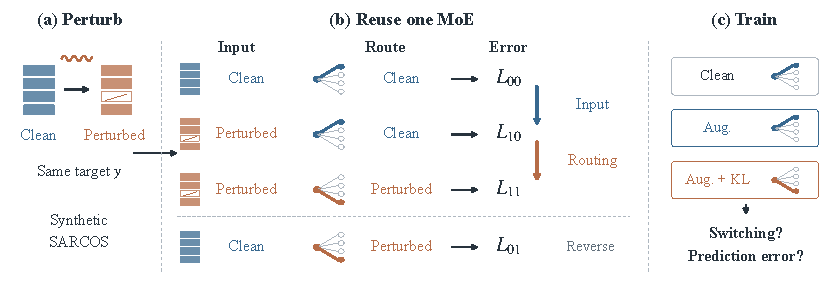
\includegraphics[width=\linewidth]{figures/figure1.pdf}

\caption{配对干预设计。同一训练好的 MoE 分别采用四种专家输入与路由组合。路由包含专家身份和门控权重。普通训练、数据增强、增强加路由一致性约束构成独立的训练对照，用于比较专家切换和预测误差。}

\label{fig:design1}

\end{figure}

\FloatBarrier

\section{相关工作}

稀疏门控混合模型、GShard、Switch Transformers、ST-MoE 和 V-MoE 将路由用于条件计算（\citealp{shazeer2017}；\citealp{lepikhin2021}；\citealp{fedus2022}；\citealp{zoph2022}；\citealp{riquelme2021}）。BASE layers、hash layers 和 expert-choice routing 提供了其他专家分配机制（\citealp{lewis2021}；\citealp{roller2021}；\citealp{zhou2022}）。负载均衡目标可能影响专家专门化（\citealp{chen2022}；\citealp{qiu2025}）。\citet{puigcerver2022}研究了对抗鲁棒性与路由、专家差异之间的联系。


专家切换频率和负载均衡描述的是分配行为，不能直接测量路由变化对预测误差的贡献。本文借鉴直接效应与交换干预分解的思路（\citealp{pearl2001}；\citealp{geiger2021}），在固定模型内部对专家输入和路由实施四格配对干预。这些对比依赖所选干预路径；当输入与路由发生交互时，它们不构成唯一、与顺序无关的误差归因。


\FloatBarrier

\section{实验设计与干预方法}

\subsection{合成任务与训练分布}

每个合成输入为 $x=(e_c,u,v,m)$，共 28 维。任务类别 c 属于 \{1, 2, 3, 4\}；$e_{c}$ 是四维独热任务提示；u 和 v 分别是八维预测特征和无关特征；m 是八维二元缺失指示变量。预测特征 u 的各坐标独立服从标准正态分布，且与任务类别无关。在加入捷径偏移之前，无关特征 v 也独立服从标准正态分布，并与 u 和 c 相互独立。


任务提示决定由以下哪个函数生成目标，因此任务变化改变的是预测映射，而不是 u 的分布。按任务标准化之前，四个函数为：


\[
f_1(u)=\frac{\sum_{i=1}^{8}u_i}{\sqrt{8}}
\]

\[
f_2(u)=\frac{\sum_{i=1}^{4}u_i-\sum_{i=5}^{8}u_i}{\sqrt{8}}
\]

\[
f_3(u)=\frac{u_1u_2+u_3u_4}{\sqrt{2}}
\]

\[
f_4(u)=\sin\left(\frac{\sum_{i=1}^{8}u_i}{\sqrt{8}}\right)
\]

前两个任务对应不同的线性方向，第三个需要乘性交互，第四个在第一个任务使用的投影上施加正弦函数。目标为 $y=(f_c(u)-\mu_c)/\sigma_c$，其中均值和标准差均由训练数据计算。按任务标准化使四类任务的均方误差处于可比较尺度。


训练、验证和测试集分别包含 80,000、10,000 和 20,000 个样本，各任务均衡。数据生成种子分别为 10,000、20,000 和 30,000，优化种子 0--4 共用这些划分。缺失指示变量在训练时始终为零；遮挡评估时，要么继续保持为零，要么标记被遮挡坐标。


独立分布条件中的无关特征不带任务偏移。捷径分布条件在训练和验证时，向前四个无关坐标加入 $2e_c$；测试时移除该偏移。两种条件均保留显式任务提示。因此，捷径条件下的干净测试本身已移除训练捷径，后续噪声和平移干预均相对于这一干净测试条件进行配对比较。


\subsection{模型与优化}

路由器为 28 \ensuremath{\rightarrow} 128 \ensuremath{\rightarrow} 4 的多层感知机，隐藏层使用 Tanh，输出为 softmax。四个专家均为 28 \ensuremath{\rightarrow} 128 \ensuremath{\rightarrow} 128 \ensuremath{\rightarrow} 1 的网络，隐藏层使用 ReLU。令 j(x) 为所选专家，w(x) 为其 softmax 权重，则预测为 $w(x)h_{j(x)}(x)$。每次仅执行所选专家；top-1 选择后保留原门控权重，不将其重新归一化为 1。


训练目标为均方误差加负载均衡损失 $0.1\times4\sum_e F_e\bar p_e$，其中 $F_{e}$ 是专家 e 在小批量中的选择频率，$\bar p_e$ 是其平均路由概率。所有模型训练 100 个 epoch，批大小为 1,024，采用 AdamW，固定学习率 0.002，权重衰减 $10^{-4}$。根据干净验证集最低 MSE 选择检查点。


MoE 含 85,640 个参数，每个样本执行 24,192 次活跃线性乘加运算（MAC）。计算量匹配的稠密网络为 28 \ensuremath{\rightarrow} 139 \ensuremath{\rightarrow} 145 \ensuremath{\rightarrow} 1，含 24,477 个参数和 24,192 次线性 MAC。参数量匹配的网络为 28 \ensuremath{\rightarrow} 206 \ensuremath{\rightarrow} 383 \ensuremath{\rightarrow} 1，含 85,639 个参数和 85,049 次线性 MAC。两种稠密模型均使用 ReLU，并采用相同的优化与检查点选择规则。这里匹配的是线性运算数量，不代表实测延迟相同。


\subsection{四格误差分解}

令 $x_{0}$ 为干净输入，$x_{1}$ 为其配对扰动输入，目标 y 保持不变。路由 $g(x)=(j(x),w(x))$ 同时包含专家身份和门控幅度。定义：


\[
L_{ab}=\mathbb{E}[(F(x_a;g(x_b))-y)^2],\quad a,b\in\{0,1\}
\]

\[
F(x_a;g(x_b))=w(x_b)h_{j(x_b)}(x_a)
\]

$L_{00}$ 是干净评估，$L_{11}$ 是通常的扰动评估。$L_{10}$ 将扰动输入交给干净路由所选的专家，并保留干净门控权重；$L_{01}$ 则使用扰动路由处理干净输入。


正向路径先改变专家输入，再改变路由：


\[
\Delta=L_{11}-L_{00}=A+R
\]

\[
A=L_{10}-L_{00},\qquad R=L_{11}-L_{10}
\]

A 为正，表示固定干净路由时，专家输入变化增加误差。R 为正，表示在扰动输入上采用新路由进一步增加误差；R 为负，则表示新路由起补偿作用。在扰动输入上恢复干净路由所造成的误差变化为 -R，因此 R 为正时恢复有利，R 为负时恢复反而有害。


反向路径先改变路由，其路由项和输入项分别为 $L_{01}$ - $L_{00}$ 与 $L_{11}$ - $L_{01}$。交互项定义为：


\[
I=L_{11}-L_{10}-L_{01}+L_{00}
\]

\[
\mathrm{Reverse\ routing}=R-I,\quad\mathrm{Reverse\ input}=A+I
\]

当 I 非零时，两条路径对同一总变化给出不同的分配。除非另有说明，后文的``输入''和``路由''均指正向路径效应。该路径下的输入主导不能自动解释为与顺序无关的重要性排序。这些是模型内部的干预对比，也不意味着干净路由一定最优。


\subsection{扰动与不确定性估计}

无关特征扰动包括高斯噪声 $v'=v+\epsilon$，其中 epsilon 服从 $\mathcal N(0,s^2I_8)$，以及对全部八个无关坐标施加 $v'_i=v_i+s$ 的均值平移。强度为 $s=0.25,0.5,1$，预测特征和任务提示均保留。信息丢失测试均匀随机遮挡一、二或四个预测坐标，将其置零，或在 25\%、50\%、75\% 的样本上将任务提示置零。遮挡指示变量可以保持为零，也可以在测试时激活。所有测试保持目标不变。


专家切换率为配对样本中 top-1 专家发生变化的比例。门控熵为 softmax 分布的平均香农熵，单位为 nat，最大值 log(4) \ensuremath{\approx} 1.386。最大负载为测试集上最大的专家选择频率。仅身份恢复对照固定扰动门控权重，只恢复干净专家索引。


随机扰动采用三次匹配抽样，并在源样本内部取平均；均值平移为确定性干预。对于固定数据划分，使用 1,000 次配对交叉 bootstrap，对训练种子编号与源样本编号重采样，计算百分位法 95\% 区间。同一次源样本重采样跨种子及模型比较共享。区间包含零表示该比较未确立明确的效应方向，不等于证明效应为零或方法等价。


\FloatBarrier

\section{将专家专门化作为辅助诊断}

在独立分布条件下，每类任务的主导专家平均获得该任务 0.579 的干净路由。移除这一专家后，模型转向剩余概率最高的专家，同时保留原所选门控权重。该操作使 MSE 增加 0.326，区间为 [0.089, 0.694]。固定相同权重，强制使用其余三个专家之一，并对任务和种子取平均，得到 MSE 1.310。这说明专家并非完全可互换。不同种子中的专家编号不具有天然对应关系，不能直接跨种子对齐。


\begin{figure}[!htbp]

\centering

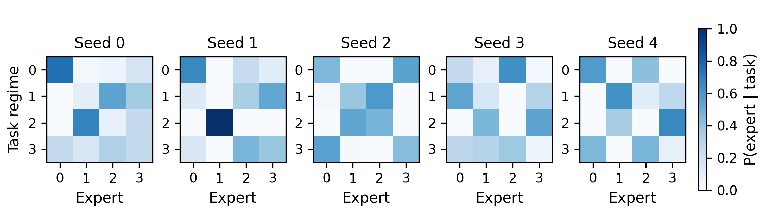
\includegraphics[width=\linewidth]{figures/figure2.pdf}

\caption{独立分布条件下各训练种子的路由矩阵。专家列仅对应各自的训练种子。}

\label{fig:design2}

\end{figure}

在 20 个种子与任务组合上，主导专家移除代价与扰动总 MSE 变化之间的 Pearson 相关系数分别为：强度 1 噪声 0.11，强度 1 均值平移 0.10，指示变量关闭时的 25\% 遮挡 0.41，50\% 任务提示删除 -0.33。这些是描述性相关。虽然移除主导专家的代价较大，但它与噪声及平移退化的联系较弱。因此，专门化程度不能替代每个扰动条件下对输入效应与路由效应的直接比较。


\FloatBarrier

\section{保留预测信息的扰动}

噪声与均值平移只作用于无关坐标，保留预测特征和任务提示。这些实验检验：在没有删除任务信息时，误差是否仍会增加，以及路由变化是否参与这一增加。表 1 报告绝对 MSE；表 2 报告相对于配对干净评估的误差变化，并乘以 10,000 以便阅读。因此，表 2 中的 1.49 表示误差变化 0.000149，而表 1 中的 0.000838 是未经缩放的误差水平。


\begin{table}[!htbp]
\centering
\caption{五个训练种子上的绝对测试 MSE 均值。噪声与平移强度均为 1；遮挡删除 25\% 预测坐标且关闭指示变量；任务提示在 50\% 样本上删除。扰动前测试无关特征均无捷径偏移。MAC 和 Param 分别表示计算量匹配与参数量匹配的稠密网络。}
\label{tab:results1}
\small
\setlength{\tabcolsep}{4pt}
\renewcommand{\arraystretch}{1.1}
\sbox{\reporttablebox}{%
\begin{tabular}{@{}llrrr@{}}
\toprule
分布 & 条件 & MoE & 稠密 MAC & 稠密 Param \\
\midrule
独立 & 干净 & 0.000698 & 0.000636 & 0.000540 \\
独立 & 噪声 & 0.000838 & 0.000690 & 0.000596 \\
独立 & 平移 & 0.000849 & 0.000671 & 0.000610 \\
独立 & 遮挡 25\% & 0.322864 & 0.322765 & 0.322870 \\
独立 & 提示删除 50\% & 0.432599 & 0.400901 & 0.349836 \\
捷径 & 干净 & 0.000748 & 0.000840 & 0.000758 \\
捷径 & 噪声 & 0.001262 & 0.001075 & 0.000955 \\
捷径 & 平移 & 0.000751 & 0.000802 & 0.000813 \\
捷径 & 遮挡 25\% & 0.322852 & 0.323029 & 0.322856 \\
捷径 & 提示删除 50\% & 0.475609 & 0.383032 & 0.349046 \\
\bottomrule
\end{tabular}}
\ifdim\wd\reporttablebox>\linewidth
\resizebox{\linewidth}{!}{\usebox{\reporttablebox}}
\else\usebox{\reporttablebox}\fi
\end{table}


\subsection{独立分布条件}

在所测试的噪声和平移强度下，正向输入项均为正，且区间不包含零。正向路由项较小，区间均包含零。噪声强度为 1 时，输入效应和路由效应按表 2 单位分别为 1.49 和 -0.10。这支持正向路径下的输入主导，但不能据此断言路由效应严格为零。


尽管如此，专家切换率仍随扰动强度增加：噪声下由 0.0057 升至 0.0235，均值平移下由 0.0072 升至 0.0274。最大负载保持在 0.254--0.258。也就是说，可以观察到专家切换，同时未检出明确的正向路由误差贡献。


\begin{table}[!htbp]
\centering
\caption{无关特征扰动下的正向分解。所有效应及区间端点均为 MSE 变化乘以 10,000。方括号为配对 95\% 区间；A 为输入项，R 为路由项，I 为交互项。}
\label{tab:results2}
\small
\setlength{\tabcolsep}{4pt}
\renewcommand{\arraystretch}{1.1}
\sbox{\reporttablebox}{%
\begin{tabular}{@{}llrrrr@{}}
\toprule
分布与扰动 & 强度 & 输入 A & 路由 R & 交互 I & 总变化 \\
\midrule
\makecell[l]{独立噪声} & 0.25 & \makecell[r]{0.07\\{}[0.04, 0.10]} & \makecell[r]{0.01\\{}[-0.03, 0.05]} & \makecell[r]{-0.05\\{}[-0.08, -0.03]} & \makecell[r]{0.08\\{}[0.04, 0.13]} \\
\makecell[l]{独立噪声} & 0.50 & \makecell[r]{0.34\\{}[0.23, 0.49]} & \makecell[r]{-0.04\\{}[-0.15, 0.05]} & \makecell[r]{-0.19\\{}[-0.30, -0.12]} & \makecell[r]{0.30\\{}[0.18, 0.49]} \\
\makecell[l]{独立噪声} & 1 & \makecell[r]{1.49\\{}[1.02, 2.10]} & \makecell[r]{-0.10\\{}[-0.41, 0.13]} & \makecell[r]{-0.88\\{}[-1.43, -0.51]} & \makecell[r]{1.40\\{}[0.91, 1.95]} \\
\makecell[l]{独立平移} & 0.25 & \makecell[r]{0.11\\{}[0.05, 0.19]} & \makecell[r]{-0.02\\{}[-0.11, 0.11]} & \makecell[r]{-0.05\\{}[-0.08, -0.03]} & \makecell[r]{0.10\\{}[-0.03, 0.22]} \\
\makecell[l]{独立平移} & 0.50 & \makecell[r]{0.40\\{}[0.25, 0.55]} & \makecell[r]{-0.03\\{}[-0.20, 0.17]} & \makecell[r]{-0.19\\{}[-0.27, -0.12]} & \makecell[r]{0.37\\{}[0.10, 0.64]} \\
\makecell[l]{独立平移} & 1 & \makecell[r]{1.60\\{}[1.14, 2.13]} & \makecell[r]{-0.10\\{}[-0.42, 0.32]} & \makecell[r]{-0.69\\{}[-1.00, -0.37]} & \makecell[r]{1.50\\{}[0.85, 2.40]} \\
\midrule
\makecell[l]{捷径噪声} & 0.25 & \makecell[r]{0.24\\{}[0.15, 0.34]} & \makecell[r]{-0.04\\{}[-0.11, 0.02]} & \makecell[r]{-0.17\\{}[-0.25, -0.11]} & \makecell[r]{0.20\\{}[0.09, 0.32]} \\
\makecell[l]{捷径噪声} & 0.50 & \makecell[r]{1.15\\{}[0.92, 1.51]} & \makecell[r]{-0.11\\{}[-0.42, 0.26]} & \makecell[r]{-0.68\\{}[-1.03, -0.41]} & \makecell[r]{1.04\\{}[0.69, 1.57]} \\
\makecell[l]{捷径噪声} & 1 & \makecell[r]{5.31\\{}[4.32, 6.31]} & \makecell[r]{-0.17\\{}[-1.49, 1.18]} & \makecell[r]{-2.55\\{}[-4.14, -1.38]} & \makecell[r]{5.14\\{}[3.68, 6.83]} \\
\makecell[l]{捷径平移} & 0.25 & \makecell[r]{-0.16\\{}[-0.46, 0.07]} & \makecell[r]{-0.24\\{}[-0.38, -0.14]} & \makecell[r]{-0.25\\{}[-0.58, -0.06]} & \makecell[r]{-0.40\\{}[-0.73, -0.21]} \\
\makecell[l]{捷径平移} & 0.50 & \makecell[r]{0.20\\{}[-0.36, 0.95]} & \makecell[r]{-0.68\\{}[-1.26, -0.28]} & \makecell[r]{-1.00\\{}[-2.25, -0.21]} & \makecell[r]{-0.48\\{}[-0.84, -0.20]} \\
\makecell[l]{捷径平移} & 1 & \makecell[r]{2.33\\{}[0.51, 5.13]} & \makecell[r]{-2.29\\{}[-4.88, -0.61]} & \makecell[r]{-3.93\\{}[-8.78, -0.82]} & \makecell[r]{0.04\\{}[-0.47, 0.53]} \\
\bottomrule
\end{tabular}}
\ifdim\wd\reporttablebox>\linewidth
\resizebox{\linewidth}{!}{\usebox{\reporttablebox}}
\else\usebox{\reporttablebox}\fi
\end{table}


\subsection{捷径分布条件与路由补偿}

捷径训练模型在噪声下表现出更大的正向输入效应，路由区间仍包含零。均值平移则呈现不同机制：所有测试强度下 R 均为负，且区间均低于零。因此，在相同平移输入上，新路由相对于保留干净路由能够降低误差。


强度 0.25 和 0.5 下，总误差变化为负，输入项区间包含零。强度 1 下，输入效应为 +2.33 [0.51, 5.13]，路由效应为 -2.29 [-4.88, -0.61]，单位同表 2；总变化为 0.04 [-0.47, 0.53]。这里很小的净变化来自输入损害与路由补偿近乎抵消，而不是内部没有发生作用。切换率为 0.0067--0.0263，最大负载为 0.258--0.262。


单独移除捷径偏移、保持目标与任务提示不变，使 MoE 的 MSE 增加 0.000301 [0.000181, 0.000543]；计算量匹配稠密模型的增加为 0.000217 [0.000147, 0.000311]。这一偏移移除对比，与表 2 在干净测试基础上追加的均值平移是不同的比较。


\subsection{反向路径与归因边界}

表 3 以原始 MSE 报告反向路径。在独立分布条件下，反向路由项和输入项均低于 0.0001，但这并不意味着它与正向路径给出相同的相对归因。例如噪声强度为 1 时，先改变路由的贡献为 0.000078，而总变化约为 0.000140。这说明较小的正向路由项可以与较大的反向路由项同时存在。


\begin{table}[!htbp]
\centering
\caption{强度 1 下的反向路径均值，单位为原始 MSE。路由项先在干净专家输入上改变路由，输入项再在该路由下改变专家输入。}
\label{tab:results3}
\small
\setlength{\tabcolsep}{4pt}
\renewcommand{\arraystretch}{1.1}
\sbox{\reporttablebox}{%
\begin{tabular}{@{}llrr@{}}
\toprule
分布 & 扰动 & 先改路由 $L_{01}$ - $L_{00}$ & 后改输入 $L_{11}$ - $L_{01}$ \\
\midrule
独立 & 噪声 & 0.000078 & 0.000062 \\
独立 & 平移 & 0.000059 & 0.000091 \\
捷径 & 噪声 & 0.000238 & 0.000276 \\
捷径 & 平移 & 0.000164 & -0.000160 \\
\bottomrule
\end{tabular}}
\ifdim\wd\reporttablebox>\linewidth
\resizebox{\linewidth}{!}{\usebox{\reporttablebox}}
\else\usebox{\reporttablebox}\fi
\end{table}


在捷径平移条件下，先对干净专家输入改变路由，使 MSE 增加 0.000164；随后改变专家输入使其降低 0.000160。强度 0.25 和 0.5 下，第二项分别为 -0.000042 和 -0.000081。平移路由与平移输入组合时有利，并不意味着将它移植到干净输入上也有利。因此，正反路径描述的是不同条件下的效应，均不能支持普遍的输入与路由重要性排名。


\subsection{稠密基线与实测代价}

25\% 遮挡下，三种架构的平均误差几乎一致。任务提示删除时，两种分布条件下 MoE 的平均 MSE 均高于两种稠密基线。独立分布、噪声强度 1 下，MoE 减去计算量匹配稠密网络的配对 MSE 差为 0.000148 [-0.000200, 0.000412]；减去参数量匹配网络的差为 0.000242 [-0.000082, 0.000503]。这些区间未确立明确差异。


在单张 A800 上，批大小为 1,024 时，使用 Python 专家分派的 MoE 干净输入延迟为 1.193 ms，计算量匹配与参数量匹配稠密模型分别为 0.144 ms 和 0.145 ms。测量为 10 次预热后 30 次同步前向的中位数。该实现中，活跃线性 MAC 匹配并未带来延迟匹配。


\FloatBarrier

\section{特征遮挡与任务提示删除}

特征遮挡删除预测坐标，但保留任务提示；提示删除则移除用于确定预测映射的变量。两者均丢失信息，却不必产生相同的路由效应。


\subsection{合成遮挡下的不可约误差}

设八个预测坐标中有 k 个被遮挡，$q=k/8$，O 包含可见坐标、遮挡位置与任务提示。对任意预测器 h(O)，有：


\[
\mathbb{E}[(Y-h(O))^2]=\mathbb{E}[\mathrm{Var}(Y\mid O)]+\mathbb{E}[(\mathbb{E}[Y\mid O]-h(O))^2]
\]

第一项是信息缺失所造成的参考风险，第二项是模型高于该参考的超额预测误差。两个线性任务的原始参考风险为 q。乘积任务对均匀随机遮挡位置取平均后，原始风险为 $1-(8-k)(7-k)/56$。正弦任务中，令 $S_{o}$ 为可见坐标的归一化和，条件均值为 $e^{-q/2}\sin(S_o)$，原始参考风险为：


\[
\frac{1-e^{-2}-e^{-q}+e^{-2+q}}{2}
\]

各任务风险再除以对应训练目标方差。参考风险计算与四格分解是两种不同分析：表 4 和表 5 分解的是 $L_{11}$ - $L_{00}$，而不是模型高于参考风险的超额误差。


\subsection{合成任务遮挡}

独立分布条件下，遮挡由一个坐标增加到四个时，总 MSE 增量由约 0.167 增至 0.596。正向输入项分别为 0.160、0.313、0.588，路由项均低于 0.01。切换率由 0.121 升至 0.272，最大负载维持在 0.256--0.264。可见，较高的切换率仍可对应输入主导的正向分解。捷径条件呈现类似模式，但路由项略大。


\begin{table}[!htbp]
\centering
\caption{捷径分布下的信息丢失效应。输入、路由、总变化均为原始 MSE 增量，切换率为专家身份变化比例。遮挡指示变量保持为零。}
\label{tab:results4}
\small
\setlength{\tabcolsep}{4pt}
\renewcommand{\arraystretch}{1.1}
\sbox{\reporttablebox}{%
\begin{tabular}{@{}llrrrr@{}}
\toprule
类型 & 水平 & 输入 & 路由 & 总变化 & 切换率 \\
\midrule
遮挡 & 12.5\% & 0.160 & 0.0069 & 0.167 & 0.114 \\
遮挡 & 25\% & 0.311 & 0.0113 & 0.322 & 0.163 \\
遮挡 & 50\% & 0.581 & 0.0155 & 0.596 & 0.238 \\
提示删除 & 25\% & 0.127 & 0.107 & 0.234 & 0.166 \\
提示删除 & 50\% & 0.259 & 0.215 & 0.475 & 0.332 \\
提示删除 & 75\% & 0.389 & 0.333 & 0.722 & 0.499 \\
\bottomrule
\end{tabular}}
\ifdim\wd\reporttablebox>\linewidth
\resizebox{\linewidth}{!}{\usebox{\reporttablebox}}
\else\usebox{\reporttablebox}\fi
\end{table}


在独立条件的 25\% 遮挡下，仅恢复专家身份的收益为 -0.0034 [-0.0067, 0.0003]。这里正收益表示在固定扰动门控权重的情况下，恢复干净专家身份使 MSE 降低。因此，该条件下没有确立身份恢复能够修复预测。


缺失标记对照对相同遮挡分别关闭和开启指示变量。在 25\% 遮挡且关闭指示变量时，该配对对照的 MoE MSE 为 0.322395，经验条件均值参考 MSE 为 0.319043，超额误差为 0.003352 [0.002758, 0.003912]。表~\ref{tab:results1} 的 0.322864 来自原始的独立无标记遮挡评估。两次评估使用相同检查点和测试源样本，但遮挡抽样不同：配对对照使用种子 9015--9017，独立无标记条件使用 9024--9026，因此绝对 MSE 不必相同。训练期间指示变量始终为零，仅在测试时开启会进一步增加误差：12.5\% 遮挡时为 0.0108 [0.0082, 0.0135]，25\% 时为 0.0185 [0.0136, 0.0238]，50\% 时为 0.0261 [0.0197, 0.0325]。该对照检验的是训练与评估不匹配，不能据此评价经过训练的缺失指示变量是否有用。在 25\% 遮挡并激活指示变量时，MoE 减去计算量匹配稠密模型的 MSE 差为 -0.0231 [-0.0461, -0.0092]。


\begin{table}[!htbp]
\centering
\caption{独立分布下的信息丢失效应，单位为原始 MSE 变化。遮挡指示变量保持为零。}
\label{tab:results5}
\small
\setlength{\tabcolsep}{4pt}
\renewcommand{\arraystretch}{1.1}
\sbox{\reporttablebox}{%
\begin{tabular}{@{}llrrrr@{}}
\toprule
类型 & 水平 & 输入 & 路由 & 总变化 & 切换率 \\
\midrule
遮挡 & 12.5\% & 0.160 & 0.0067 & 0.167 & 0.121 \\
遮挡 & 25\% & 0.313 & 0.0093 & 0.322 & 0.182 \\
遮挡 & 50\% & 0.588 & 0.0078 & 0.596 & 0.272 \\
提示删除 & 25\% & 0.138 & 0.074 & 0.212 & 0.149 \\
提示删除 & 50\% & 0.283 & 0.149 & 0.432 & 0.298 \\
提示删除 & 75\% & 0.425 & 0.228 & 0.653 & 0.444 \\
\bottomrule
\end{tabular}}
\ifdim\wd\reporttablebox>\linewidth
\resizebox{\linewidth}{!}{\usebox{\reporttablebox}}
\else\usebox{\reporttablebox}\fi
\end{table}


\subsection{任务提示删除}

提示删除使两个正向项均增加。在独立分布条件下，删除比例由 25\% 增至 75\% 时，切换率由 0.149 升至 0.444。删除比例为 50\% 时，输入项为 0.283 [0.248, 0.321]，路由项为 0.149 [0.086, 0.208]。因此，在该条件下对扰动输入恢复干净路由能够降低误差。仅身份恢复的收益为 0.176 [0.105, 0.247]，支持专家选择具有重要贡献，但不能证明门控幅度完全不起作用。最大负载随提示删除比例由 0.307 升至 0.436。


捷径条件同样具有正的输入项和路由项。50\% 提示删除时，两者分别为 0.259 和 0.215。输入仍是更大的平均贡献，但路由所占比例高于独立条件。与遮挡不同，提示删除使路由变化本身在正向路径上增加误差。


干净输入上的门控熵已经较高：独立条件为 1.267，捷径条件为 1.303，最大值为 log(4) \ensuremath{\approx} 1.386。噪声、平移和零指示变量遮挡造成的熵变化均小于 0.003。75\% 提示删除时，两种条件分别升至 1.329 [1.311, 1.347] 和 1.358 [1.352, 1.364]。熵与负载描述路由如何响应，而干预对比判断这种响应是否增加误差。


\FloatBarrier

\section{将路由一致性作为补充训练检验}

前文在固定检查点下比较输入变化和路由变化的效应。本节进一步检验：显式减少路由变化，是否带来可检出的预测收益。每种分布设三个训练组：普通训练、标准差 0.5 的无关特征噪声增强，以及增强加 $0.1D_{\mathrm{KL}}(\operatorname{stopgrad}(p(x))\Vert p(\tilde x))$，其中 p 为路由 softmax。


增强组和一致性组对干净视图与噪声视图的 MSE 和均衡损失取平均，普通组使用两个相同的干净视图。各组共享对应种子的初始化、小批量顺序，并在适用时共享匹配噪声抽样，采用相同的 100 epoch 日程及干净验证集选点规则。本节普通训练对照重新训练，因此数值与表 1 不同。


\begin{table}[!htbp]
\centering
\caption{强度 1 下的匹配合成训练比较。MSE 为绝对误差且不缩放，切换率为专家身份变化比例。最后一列为一致性组减去增强组的 MSE。}
\label{tab:results6}
\small
\setlength{\tabcolsep}{4pt}
\renewcommand{\arraystretch}{1.1}
\sbox{\reporttablebox}{%
\begin{tabular}{@{}llrrrr@{}}
\toprule
分布 & 测试指标 & 普通 & 增强 & 一致性 & 一致性减增强 \\
\midrule
独立 & 噪声 MSE & 0.000899 & 0.000787 & 0.000669 & -0.000118 \\
独立 & 噪声切换率 & 0.0288 & 0.0230 & 0.0160 & --- \\
独立 & 平移 MSE & 0.000897 & 0.000731 & 0.000674 & -0.000057 \\
独立 & 平移切换率 & 0.0318 & 0.0311 & 0.0153 & --- \\
捷径 & 噪声 MSE & 0.001392 & 0.000868 & 0.000598 & -0.000270 \\
捷径 & 噪声切换率 & 0.0400 & 0.0315 & 0.0109 & --- \\
捷径 & 平移 MSE & 0.000782 & 0.000705 & 0.000440 & -0.000264 \\
捷径 & 平移切换率 & 0.0409 & 0.0256 & 0.0099 & --- \\
\bottomrule
\end{tabular}}
\ifdim\wd\reporttablebox>\linewidth
\resizebox{\linewidth}{!}{\usebox{\reporttablebox}}
\else\usebox{\reporttablebox}\fi
\end{table}


相对于普通训练，数据增强降低了平均误差。一致性组在四个强度 1 对比中均具有最低的平均误差和切换率，但一致性减增强的配对 MSE 区间全部包含零：独立条件噪声和平移分别为 [-0.000299, 0.000043]、[-0.000254, 0.000112]，捷径条件分别为 [-0.000748, 0.000023]、[-0.000641, 0.000004]。结果显示观察到的切换更少，但尚未确立相对于增强的额外精度收益，也未证明两种方法等价。


\begin{figure}[!htbp]

\centering

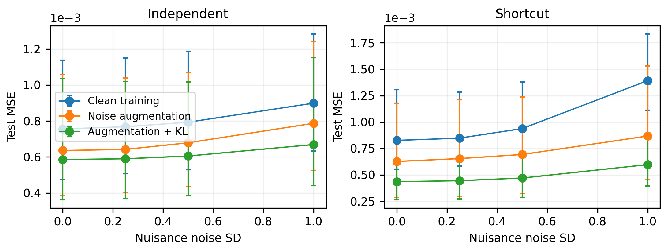
\includegraphics[width=\linewidth]{figures/figure3.pdf}

\caption{匹配训练组对合成无关特征噪声的响应。误差棒为各组均值的 95\% 区间，配对误差差值区间在正文中给出。}

\label{fig:design3}

\end{figure}

\subsection{分离专家身份与门控幅度}

路由包含两个部分，恢复它们可能产生方向相反的作用。固定标准差 1 噪声下的专家输入 z，定义：


\[
M_{ab}=\mathbb{E}[(w_b h_{j_a}(z)-y)^2]
\]

\[
(j_0,w_0)=g(x),\qquad(j_1,w_1)=g(z)
\]

\[
B_{\mathrm{ID}}=M_{11}-M_{01},\quad B_w=M_{11}-M_{10},\quad B_{\mathrm{joint}}=M_{11}-M_{00}
\]

B 为正表示恢复后 MSE 降低。各组合共享检查点、输入和三次噪声抽样。在捷径增强组，恢复干净专家身份能够降低误差，收益为 4.23 \ensuremath{\times} $10^{-5}$，区间为 [0.82, 8.99] \ensuremath{\times} $10^{-5}$；恢复干净门控权重反而增加误差，收益为 -5.65 \ensuremath{\times} $10^{-5}$，区间为 [-8.72, -2.68] \ensuremath{\times} $10^{-5}$；共同恢复的收益为 -1.51 \ensuremath{\times} $10^{-5}$，区间为 [-6.14, 3.61] \ensuremath{\times} $10^{-5}$。因此，该条件下身份恢复有利、权重恢复有害，共同恢复的效应则未明确区别于零。这两个条件恢复收益也不必相加，因为专家身份与权重可以交互。


30 个检查点均保持四个专家活跃。六个分布与训练组组合的平均最大负载为 0.258--0.277，单个检查点最大值为 0.312，没有训练组将全部选择集中到单一专家。


\FloatBarrier

\section{SARCOS 真实数据验证}

\subsection{任务与评估设计}

SARCOS 逆动力学数据提供 21 个传感器坐标，包括七个关节的位置、速度与加速度，以及七个关节力矩目标（\citealp{vijayakumar2005}）。我们每次预测一个关节力矩，并将七维独热关节提示置于 21 维传感器输入之前，构成 28 维输入，从而复用合成实验的网络结构。该提示标识当前预测任务，是实验额外加入的变量，不是原始档案中的传感器。


从开发数据中移除 4,428 条输入状态与测试状态完全相同的记录后，得到 35,056 条训练、5,000 条验证和 4,449 条测试记录，划分种子为 20261027。输入缩放与各关节目标标准化仅使用训练数据。每个 epoch 为每个训练源样本分配一个关节，每七个 epoch 遍历全部关节；验证与测试覆盖所有关节。


七种配置结合优化种子 0--4，共进行 35 次训练：三种架构各自的普通训练与增强训练，以及 MoE 的增强加一致性训练。优化设置同第 3.2 节。每个种子在不同配置间共享源样本顺序和关节分配，同一架构共享初始化。增强向标准化传感器加入标准差 0.1 的噪声，一致性系数为 0.1。


测试分别使用标准差 0.1、0.25、0.5 的传感器噪声，随机将三个或六个传感器坐标置零，或在 50\% 源样本上删除关节提示。目标保持不变，同一源样本跨关节任务共享受扰动状态。Macro-NMSE 对按训练方差归一化的平方误差在关节与源样本上取平均。在交叉 bootstrap 前，先在每个源样本内部平均三次扰动和七个关节。主要评价终点为噪声标准差 0.25 下，一致性组减去增强组的误差。


SARCOS 噪声直接作用于预测力矩所需的传感器，而合成无关噪声保留预测坐标，因此二者误差量级不能按相同扰动含义直接比较。表 7 为不缩放的绝对 macro-NMSE，与表 2 的缩放增量不同。


\begin{table}[!htbp]
\centering
\caption{五个种子上的 SARCOS macro-NMSE 均值。噪声标准差为 0.25；遮挡删除 21 个传感器坐标中的六个。切换率对应噪声标准差 0.25。}
\label{tab:results7}
\small
\setlength{\tabcolsep}{4pt}
\renewcommand{\arraystretch}{1.1}
\sbox{\reporttablebox}{%
\begin{tabular}{@{}llrrrr@{}}
\toprule
模型 & 训练 & 干净 & 噪声 0.25 & 遮挡 6/21 & 切换率 \\
\midrule
MoE & 普通 & 0.016179 & 0.114362 & 0.409034 & 0.0669 \\
稠密 MAC & 普通 & 0.018466 & 0.124025 & 0.441438 & --- \\
稠密 Param & 普通 & 0.015070 & 0.117297 & 0.434594 & --- \\
MoE & 增强 & 0.017630 & 0.075124 & 0.307793 & 0.0660 \\
稠密 MAC & 增强 & 0.019639 & 0.085397 & 0.339033 & --- \\
稠密 Param & 增强 & 0.015967 & 0.075076 & 0.318832 & --- \\
MoE & 增强加 KL & 0.017667 & 0.075180 & 0.306018 & 0.0609 \\
\bottomrule
\end{tabular}}
\ifdim\wd\reporttablebox>\linewidth
\resizebox{\linewidth}{!}{\usebox{\reporttablebox}}
\else\usebox{\reporttablebox}\fi
\end{table}


\subsection{输入损害与路由补偿}

噪声标准差为 0.25 时，普通训练 MoE 的正向输入效应为 0.097793 [0.094766, 0.100639]，路由效应为 0.000390 [-0.000661, 0.001534]。因此，该路径下总变化主要由输入项解释。虽然切换率达到 0.0669，但未检出明确的正向路由贡献。


六坐标遮挡与合成遮挡不同：输入项为 0.425050，路由项为 -0.032195 [-0.043868, -0.020455]。新路由部分抵消输入损害，但没有消除整体退化。相对于允许模型重新路由，恢复干净路由反而会增加误差。提示删除则产生正的输入项和路由项，分别为 0.390242 和 0.016638，均值方向与合成提示删除一致；此处未报告 SARCOS 提示删除路由项的区间。


\begin{figure}[!htbp]

\centering

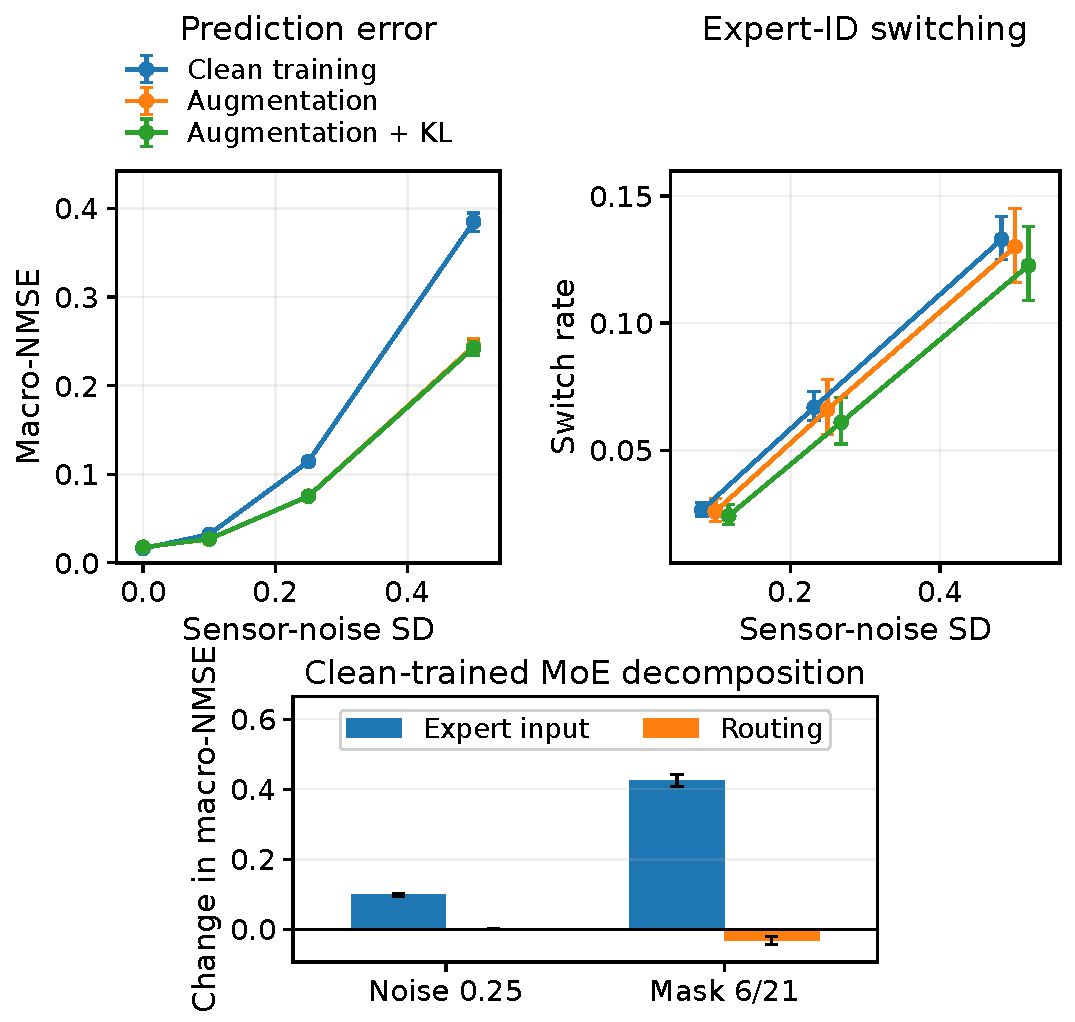
\includegraphics[width=\linewidth]{figures/figure4.pdf}

\caption{SARCOS 三个 MoE 训练组的噪声响应曲线，以及普通训练 MoE 的正向分解。误差棒为 95\% 交叉 bootstrap 区间。}

\label{fig:design4}

\end{figure}

\subsection{训练对比}

噪声标准差为 0.25 时，数据增强将 MoE 的平均 macro-NMSE 从 0.114362 降至 0.075124；加入一致性后为 0.075180。配对的一致性减增强差值为 0.000056 [-0.000928, 0.001403]，因此主要终点未确立额外的误差降低。


切换率由 0.0660 降至 0.0609，配对差值为 -0.005071 [-0.008952, -0.001401]。六坐标遮挡下，预测误差差值为 -0.001774 [-0.005062, 0.001536]，也包含零。所有 MoE 检查点均保持四个专家活跃。因此，SARCOS 支持将已检出的切换减少，与尚未确立的额外精度收益区分开来。


\FloatBarrier

\section{局限性}

合成任务的映射由人工指定，并显式提供任务提示，其专门化问题比从原始输入中发现任务边界更容易。SARCOS 的关节提示也由实验额外加入。SARCOS 将评估扩展到合成目标函数之外，但并未消除模型对显式任务标识的依赖。


模型是四个小型 MLP 专家的 top-1 混合，并保留标量 softmax 门控。结果不能直接推广到大型稀疏语言或视觉模型、top-k 路由、expert-choice 路由或其他门控约定。稠密基线来自同一前馈网络家族，分派延迟也依赖具体实现。


合成无关扰动效应常为 $10^{-4}$ 量级，而绝对 MSE 约为 $10^{-3}$。部分方向有区间支持，但实际误差变化仍较小。五个种子、单一模型规模和固定数据划分限制了推断范围。区间包含零不能证明没有效应、方法等价，或一致性训练在其他条件下不可能有效。


交互非零时，分解依赖干预路径。正向输入主导的结果可以与更大的反向路由贡献同时存在。除非显式分离，路由对比还同时包含专家身份与门控幅度。因此，解释``输入效应''和``路由效应''时必须保留对应干预定义。


扰动包括各向同性噪声、常数均值平移、随机坐标遮挡与任务提示删除，均非对抗扰动；除 SARCOS 坐标遮挡外，也未针对某一具体传感器故障设计。测试保持目标不变，研究的是观测受损条件下的预测，而不是底层物理状态变化后目标如何变化。


SARCOS 仅涉及一个机械臂和一个公开档案。移除开发集中与测试输入完全重复的记录后，分析将源记录视为独立，忽略原始轨迹中的依赖。源样本内平均处理了共享关节任务和扰动抽样，但未处理不同轨迹记录之间的相关性。


\FloatBarrier

\section{讨论与结论}

本文研究扰动引起的误差变化如何分配给专家输入与路由，以及路由变化是在加剧还是缓解损害。答案随所测试的扰动情景变化。在指定的正向路径上，合成数据与 SARCOS 的噪声退化主要体现为输入效应，未检出明确的路由贡献；删除任务提示使两个效应均增加误差；合成遮挡由输入主导，SARCOS 传感器遮挡则产生有利的新路由；最大捷径平移下，输入损害与路由补偿几乎抵消。


这些结果并未给出两种机制的统一排名，而是说明比较时必须交代扰动对象和干预路径。较小的净误差变化可能掩盖方向相反的内部效应，较高的切换率也可能对应有害、较小或有利的路由贡献。恢复干净路由同样依赖情景：在提示删除下能够降低误差，而在新路由起补偿作用的捷径平移和 SARCOS 遮挡下，恢复反而增加误差。


专家专门化与路由一致性是辅助诊断，不能替代这一分解。移除主导专家代价较大，但其代价与噪声和平移退化的联系较弱。一致性训练减少了合成实验中观察到的切换，并在 SARCOS 主要条件下产生区间支持的切换降低；其配对误差区间则未确立相对于增强的额外精度收益。进一步分离专家身份与门控幅度还表明，恢复其中一部分可能有利，恢复另一部分却可能有害。


在本文测试的条件下，输入效应与路由效应的相对大小和方向取决于扰动情景。路由变化既可能加剧预测退化，也可能缓解退化。因此，评价 MoE 的扰动鲁棒性，应在明确扰动与干预条件的前提下直接比较两种效应，而不能仅凭专家切换频率推断路由损害。


\FloatBarrier

\section*{作者贡献}

Do Anh Dung 构建任务、扰动、捷径分布和四格干预。Yang Jian 构建 MoE 与稠密模型、多种子训练及测量流程。Xiangli Qianhui 计算误差分解、bootstrap 区间、路由统计并撰写报告。AI 工具辅助文献检索、实现与写作。


\FloatBarrier

\nocite{*}

\bibliographystyle{iclr2026_conference}

\bibliography{references}

\end{document}